%%%%%%%%%%%%%%%%%%%%% chapter2.tex %%%%%%%%%%%%%%%%%%%%%%%%%%%%%%%%%
%
%  Monotone Circuits Lower bounds 
%
% Use this file as a template for your own input.
%
%%%%%%%%%%%%%%%%%%%%%%%% Springer-Verlag %%%%%%%%%%%%%%%%%%%%%%%%%%
%\motto{Use the template \emph{chapter.tex} to style the various elements of your chapter content.}





\chapter{Monotone Circuit Lower Bounds}
\label{sec:Razborov} % Always give a unique label
% use \chaptermark{}
% to alter or adjust the chapter heading in the running head


% Always give a unique label
% and use \ref{<label>} for cross-references
% and \cite{<label>} for bibliographic references
% use \sectionmark{}
% to alter or adjust the section heading in the running head

We've seen that proving that SAT is not in $P/poly$, i.e., can't be solved by polynomial-size circuits, implies that $P \neq NP$.
Due to the notorious difficulty of these questions, weare interested in proving \emph{weaker} lower bounds, namely, some lower bounds against restricted classes of circuits. 
Here, we study such a restricted circuit class: A boolean circuit without negation gates, i.e., monotone circuits.

\begin{definition}[Monotone circuit]
A Monotone circuit is a Boolean circuit that contains fan-in two gates AND and OR, but has \emph{no} NOT gates.
\end{definition}

This means in particular that monotone circuits can compute only monotone functions: a Boolean function is is said to be monotone if increasing the number of ones in the input cannot flip the value of the function from 1 to 0. 

More precisely, for $\bar{x}, \bar{y} \in\{0,1\}^n$, write $\bar{x} \geqslant \bar{y}$ iff $ \forall i \in [n], x_i \geqslant y_i$, where $[n]$ denotes $\{1,\dots,n\}$. (Here, $x_i\ge y_i$ for Boolean $x_i,y_i$ means simply that $1\ge 0$ and $0\ge 0$, $1\ge 1$, while $0\not\ge 1$.)

\begin{definition}[Monotone function]
A Boolean function $f:\{0,1\}^n \rightarrow\{0,1\}$ is said to be  \emph{monotone} if $\forall \bar{x} \geq \bar{y}, f(\bar{x}) \geqslant f(y)$.
\end{definition}


Many NP problems are monotone, like CLIQUE:

Given an undirected graph $G=(V, E)$ with $n$ nodes, a $k$-clique in $G$ is a set $U\subseteq V$ of size $k$, st. every pair of nodes $u_1, u_2 \in U$ is connected by an edge (in $E$):

$$
 \forall u_1 \in u \forall u_2 \in u ( u \neq u_2\Rightarrow (u_1, u_2)\in E).
$$


Recall that a computational (decision) problem is a \emph{language}, namely an infinite set of finite strings over a finite alphabet (usually the alphabet $\{0,1\}$), where each string encodes (in some natural way) an accepted graph, i.e., a $k$-clique with $n$ nodes.

We are interested in CLIQUE $(k, n)$ for a fixed $k$, as the following Boolean function:  a graph  $G=(V, E) $ w / $n$ nodes, is encoded by $\binom{n}{2}$ input gates $x_{ij}$, where $x_{i j}=1$ iff $(i, j) \in E$.

\begin{svgraybox}
The computational problem \textbf{CLIQUE $(k, n)$:}  

Input: Graph w/ $n$ nodes and a number $k$

Accept if the graph contains a $k$-clique. Reject otherwise.
\end{svgraybox}


 Note that $\operatorname{CLIQUE}(k, n)$ is a monotone function: If we add 1's to the input, we only increase the chance it has a k-clique! CLIQUE $(k, n)$ is NP - complete.


Since CLIQUE$(n, k)$ is a monotone (Boolean)
function we can compute it by a monotone Boolean circuit.
\medskip 

\textbf{Example of a monotone circuit computing CLIQUE$(n, k)$:} ``run" over all $\binom{n}{k} ~~ k$-sub-graphs in $G$, and check if at least one of those is a clique:

\begin{figure}
    \centering
    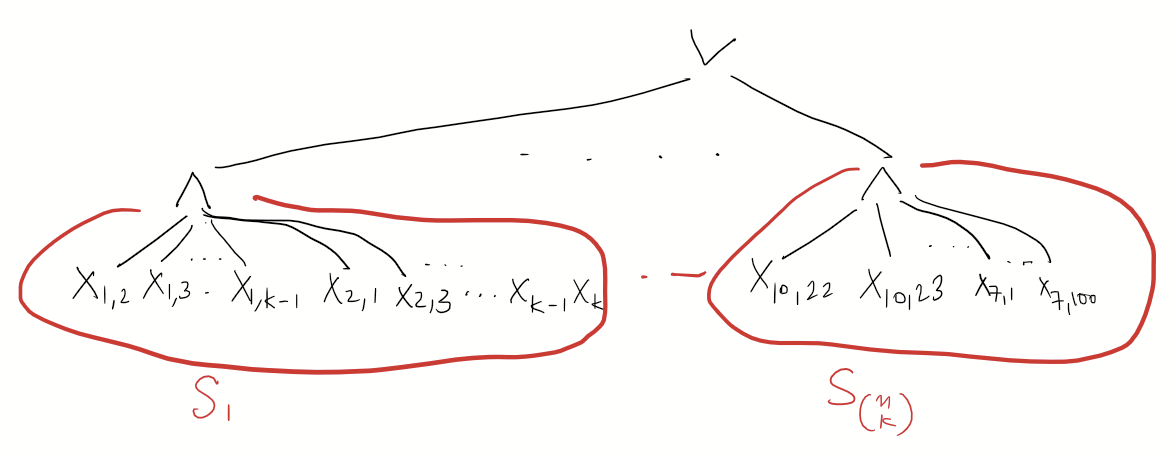
\includegraphics[width=0.75\linewidth]{images/k-clique-simple-circuit.png}
    \label{fig:enter-label}
\end{figure}





$S_1, S_2, \ldots, S_{\binom{n}{k}}$ are the $\binom{n}{k}$ subgraphs in $G$ each of size $k$.
Size of this circuit: $O\left(k^2 \cdot\binom{n}{k}\right)$.
We call such a circuit for computing $\operatorname{CLIQUE}  (n, k)$ consisting of a big $\lor$ of all $S_i$'s, each computed by $\land$'s, a \textbf{\textit{crude-circuit}} for CLIQUE($n, k)$.
